\begin{figure}[htbp]
\centering
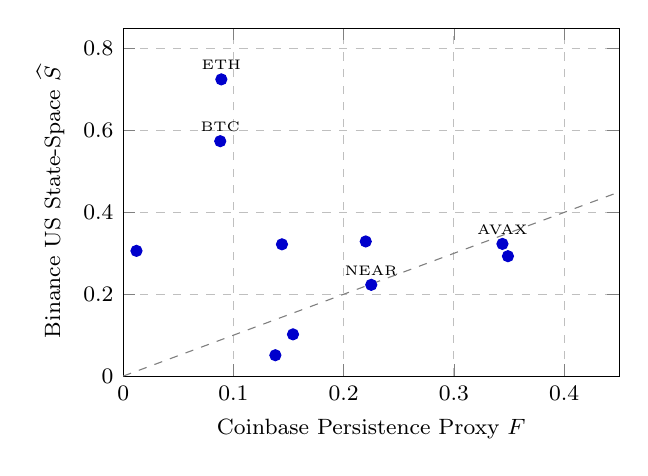
\begin{tikzpicture}
\begin{axis}[
    width=0.65\textwidth,
    height=6.0cm,
    xlabel={Coinbase Persistence Proxy $F$},
    ylabel={Binance US State-Space $\widehat S$},
    xmin=0, xmax=0.45,
    ymin=0, ymax=0.85,
    ymajorgrids=true,
    xmajorgrids=true,
    grid style=dashed,
    font=\footnotesize
]
\addplot[only marks, mark=*, color=blue!80!black] coordinates {
    (0.088, 0.574) (0.089, 0.725) (0.012, 0.306) (0.138, 0.051) (0.225, 0.223)
    (0.154, 0.102) (0.344, 0.323) (0.220, 0.329) (0.144, 0.322) (0.349, 0.293)
};
\addplot[color=gray, dashed, domain=0:0.45] {x};
\node[above, font=\tiny] at (axis cs:0.225, 0.223) {NEAR};
\node[above, font=\tiny] at (axis cs:0.344, 0.323) {AVAX};
\node[above, font=\tiny] at (axis cs:0.088, 0.574) {BTC};
\node[above, font=\tiny] at (axis cs:0.089, 0.725) {ETH};
\end{axis}
\end{tikzpicture}
\caption{Cross-exchange comparison: empirical persistence proxy $F$ on Coinbase vs.\ state-space estimate $\widehat S$ on Binance US. Divergence in high-volume pairs (BTC, ETH) illustrates noncomparability of distinct mathematical estimators rather than structural venue effects.}
\label{fig:F7_matched_venue_comparison}
\end{figure}
